% ********** Rozdział 6 **********
\chapter{Przypadki testowe}

W tej sekcji opisano przykładowe przypadki testowe dla kluczowych funkcjonalności systemu, zarówno po stronie backendu (API), jak i frontendu (interfejs użytkownika).

\section{Testy backendu (API)}

\begin{itemize}
    \item \textbf{Rejestracja nowego użytkownika}
    \begin{itemize}
        \item \textbf{Cel:} Sprawdzenie poprawności rejestracji użytkownika przez API.
        \item \textbf{Warunki początkowe:} Brak użytkownika o podanym e-mailu w bazie.
        \item \textbf{Kroki testowe:}
        \begin{enumerate}
            \item Wysłanie żądania POST /api/auth/register z danymi użytkownika.
        \end{enumerate}
        \item \textbf{Dane wejściowe:} Przykładowy e-mail, hasło, nazwa użytkownika.
        \item \textbf{Oczekiwany rezultat:} Odpowiedź 200 OK, utworzenie nowego użytkownika w bazie.
        \item \textbf{Wynik testu:}
        \begin{figure}[H]
            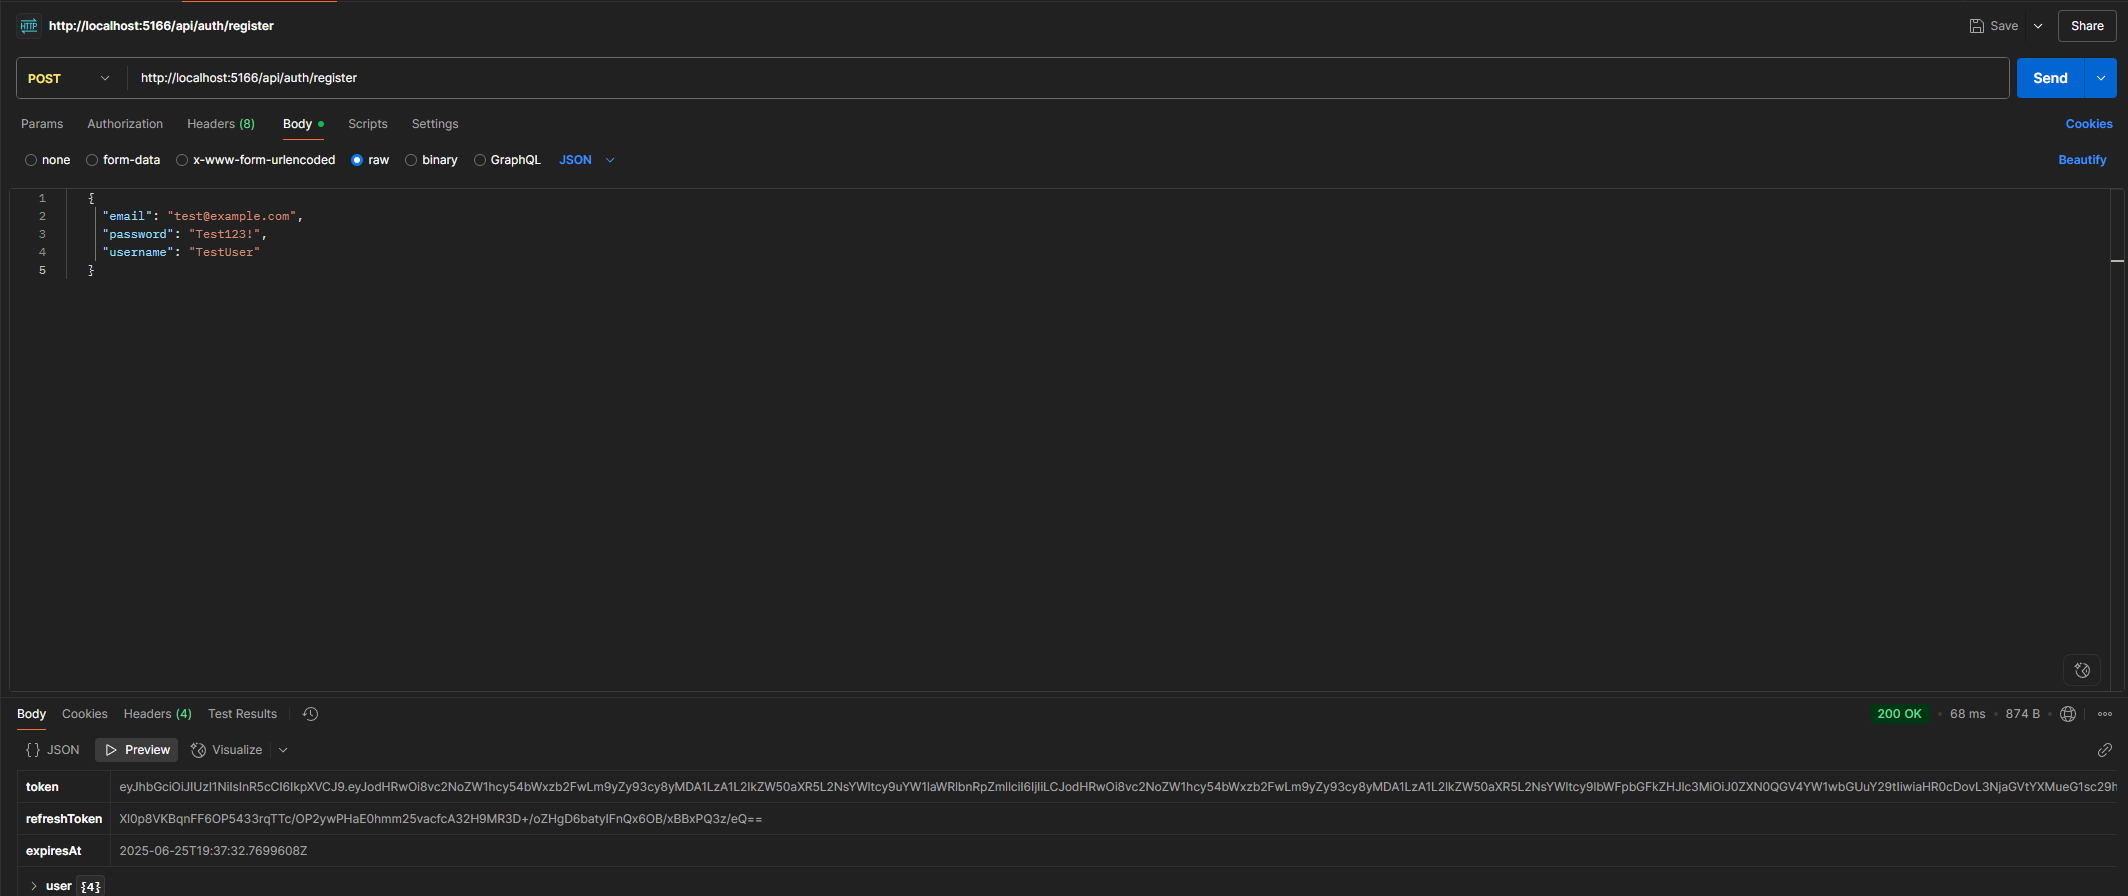
\includegraphics[width=480px]{figures/testy/test-registration.png}
            \caption{Test rejestracji użytkownika}
        \end{figure}
    \end{itemize}

    \item \textbf{Logowanie użytkownika}
    \begin{itemize}
        \item \textbf{Cel:} Sprawdzenie poprawności logowania i generowania tokenu JWT.
        \item \textbf{Warunki początkowe:} Istnieje użytkownik z podanym e-mailem i hasłem.
        \item \textbf{Kroki testowe:}
        \begin{enumerate}
            \item Wysłanie żądania POST /api/auth/login z poprawnymi danymi.
        \end{enumerate}
        \item \textbf{Dane wejściowe:} E-mail, hasło.
        \item \textbf{Oczekiwany rezultat:} Odpowiedź 200 OK, zwrócony token JWT.
        \item \textbf{Wynik testu:}
        \begin{figure}[H]
            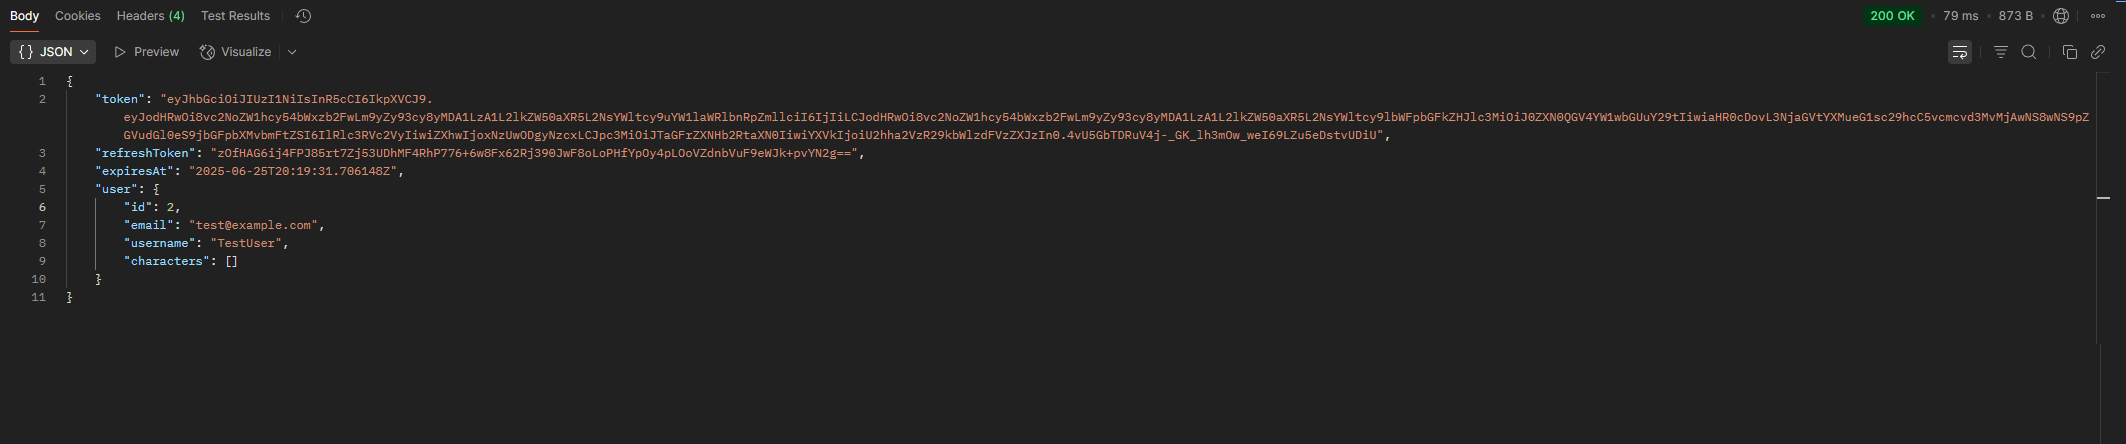
\includegraphics[width=480px]{figures/testy/test-login.png}
            \caption{Test logowania użytkownika}
        \end{figure}
    \end{itemize}

    \item \textbf{Pobranie profilu gracza}
    \begin{itemize}
        \item \textbf{Cel:} Sprawdzenie możliwości pobrania danych gracza.
        \item \textbf{Warunki początkowe:} Użytkownik jest zalogowany (ma token JWT).
        \item \textbf{Kroki testowe:}
        \begin{enumerate}
            \item Wysłanie żądania GET /api/players z nagłówkiem Authorization: Bearer <token>.
        \end{enumerate}
        \item \textbf{Dane wejściowe:} Token JWT.
        \item \textbf{Oczekiwany rezultat:} Odpowiedź 200 OK, zwrócone dane gracza.
        \item \textbf{Wynik testu:}
        \begin{figure}[H]
            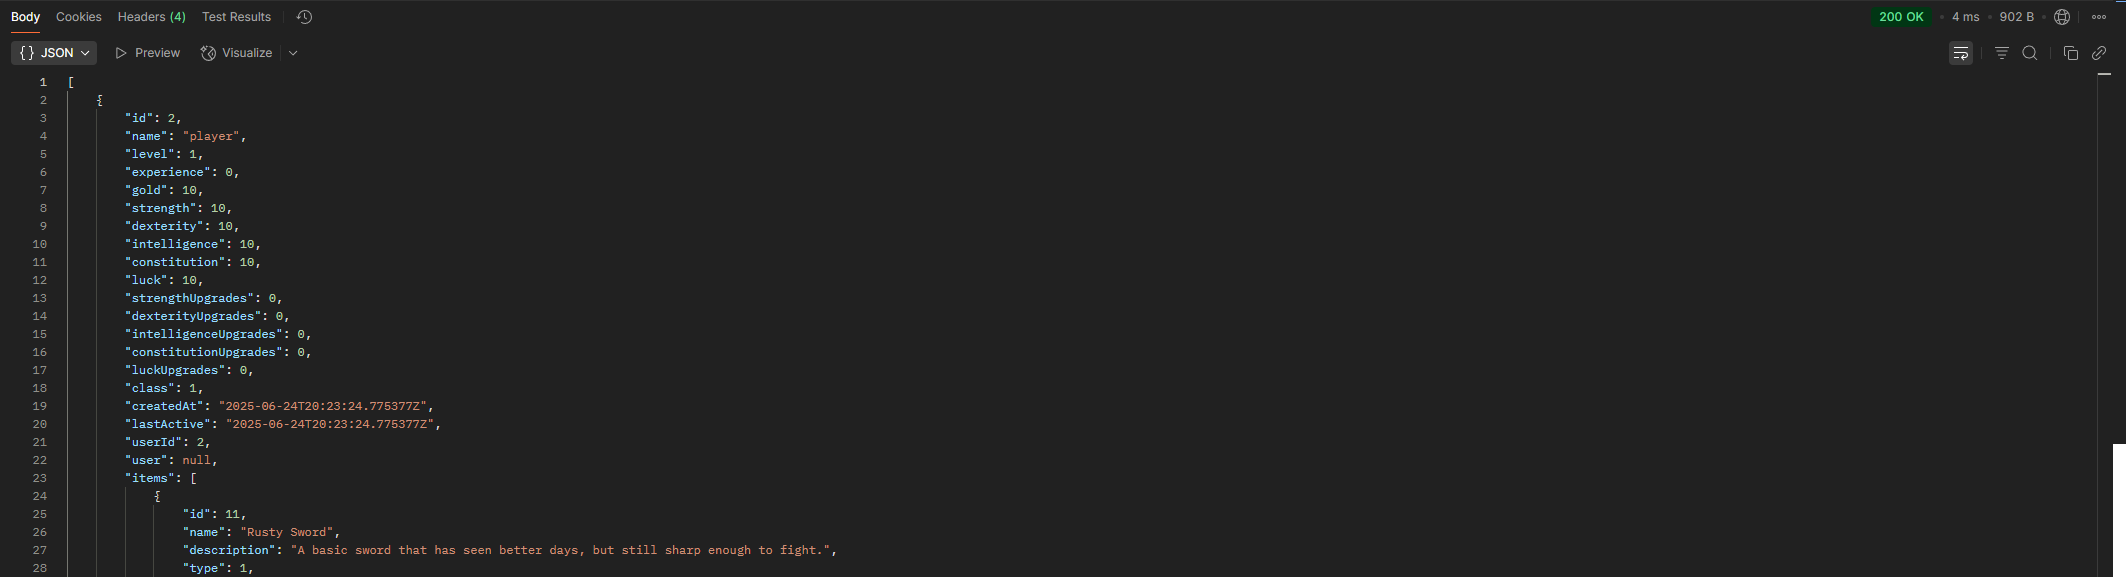
\includegraphics[width=480px]{figures/testy/test-playerdata.png}
            \caption{Test danych gracza}
        \end{figure}
    \end{itemize}

    \item \textbf{Zakup przedmiotu}
    \begin{itemize}
        \item \textbf{Cel:} Sprawdzenie możliwości zakupu przedmiotu przez API.
        \item \textbf{Warunki początkowe:} Gracz jest zalogowany, ma wystarczającą ilość złota.
        \item \textbf{Kroki testowe:}
        \begin{enumerate}
            \item Wysłanie żądania POST /api/items/buy z danymi przedmiotu.
        \end{enumerate}
        \item \textbf{Dane wejściowe:} Identyfikator przedmiotu, token JWT.
        \item \textbf{Oczekiwany rezultat:} Odpowiedź 400 Bad Request, gracz nie ma wystarczającej ilości złota.
        \item \textbf{Wynik testu:}
        \begin{figure}[H]
            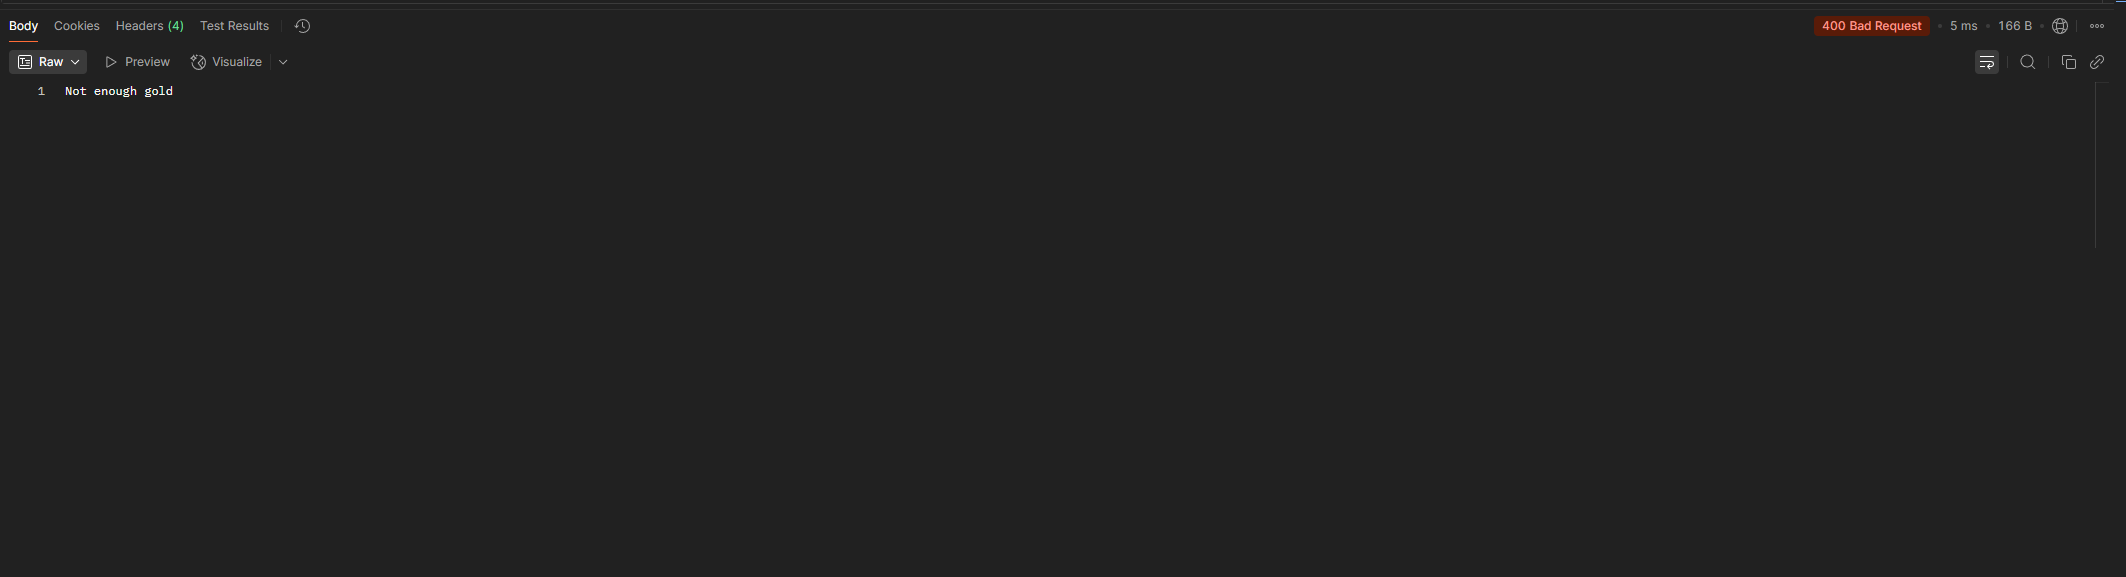
\includegraphics[width=480px]{figures/testy/test-buyitem-fail.png}
            \caption{Test zakupu przedmiotu - brak złota}
        \end{figure}
    \end{itemize}

    \item \textbf{Rozpoczęcie nowej misji}
    \begin{itemize}
        \item \textbf{Cel:} Sprawdzenie możliwości rozpoczęcia misji przez API.
        \item \textbf{Warunki początkowe:} Gracz jest zalogowany, ma dostępne misje.
        \item \textbf{Kroki testowe:}
        \begin{enumerate}
            \item Wysłanie żądania POST /api/quests/start z danymi misji.
        \end{enumerate}
        \item \textbf{Dane wejściowe:} Identyfikator misji, token JWT.
        \item \textbf{Oczekiwany rezultat:} Odpowiedź 200 OK, misja przypisana do gracza.
        \item \textbf{Wynik testu:}
        \begin{figure}[H]
            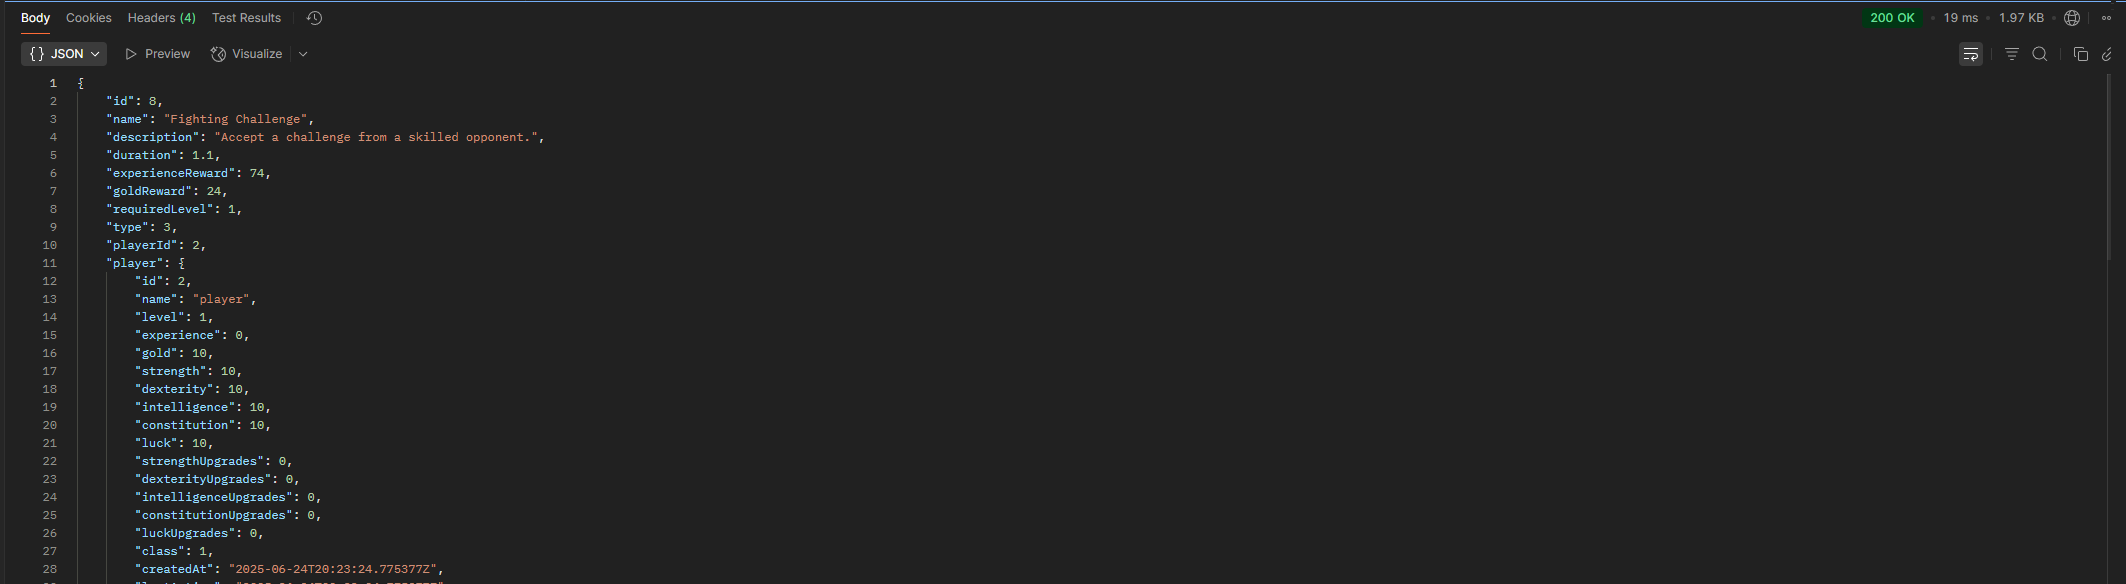
\includegraphics[width=480px]{figures/testy/test-startquest.png}
            \caption{Test rozpoczęcia misji}
        \end{figure}
    \end{itemize}

    \item \textbf{Zakończenie misji}
    \begin{itemize}
        \item \textbf{Cel:} Sprawdzenie poprawności zakończenia misji i przyznania nagrody.
        \item \textbf{Warunki początkowe:} Gracz ma aktywną misję.
        \item \textbf{Kroki testowe:}
        \begin{enumerate}
            \item Wysłanie żądania POST /api/quests/complete z danymi misji.
        \end{enumerate}
        \item \textbf{Dane wejściowe:} Identyfikator misji, token JWT.
        \item \textbf{Oczekiwany rezultat:} Odpowiedź 200 OK, nagroda dodana do ekwipunku, XP i złoto zaktualizowane.
        \item \textbf{Wynik testu:}
        \begin{figure}[H]
            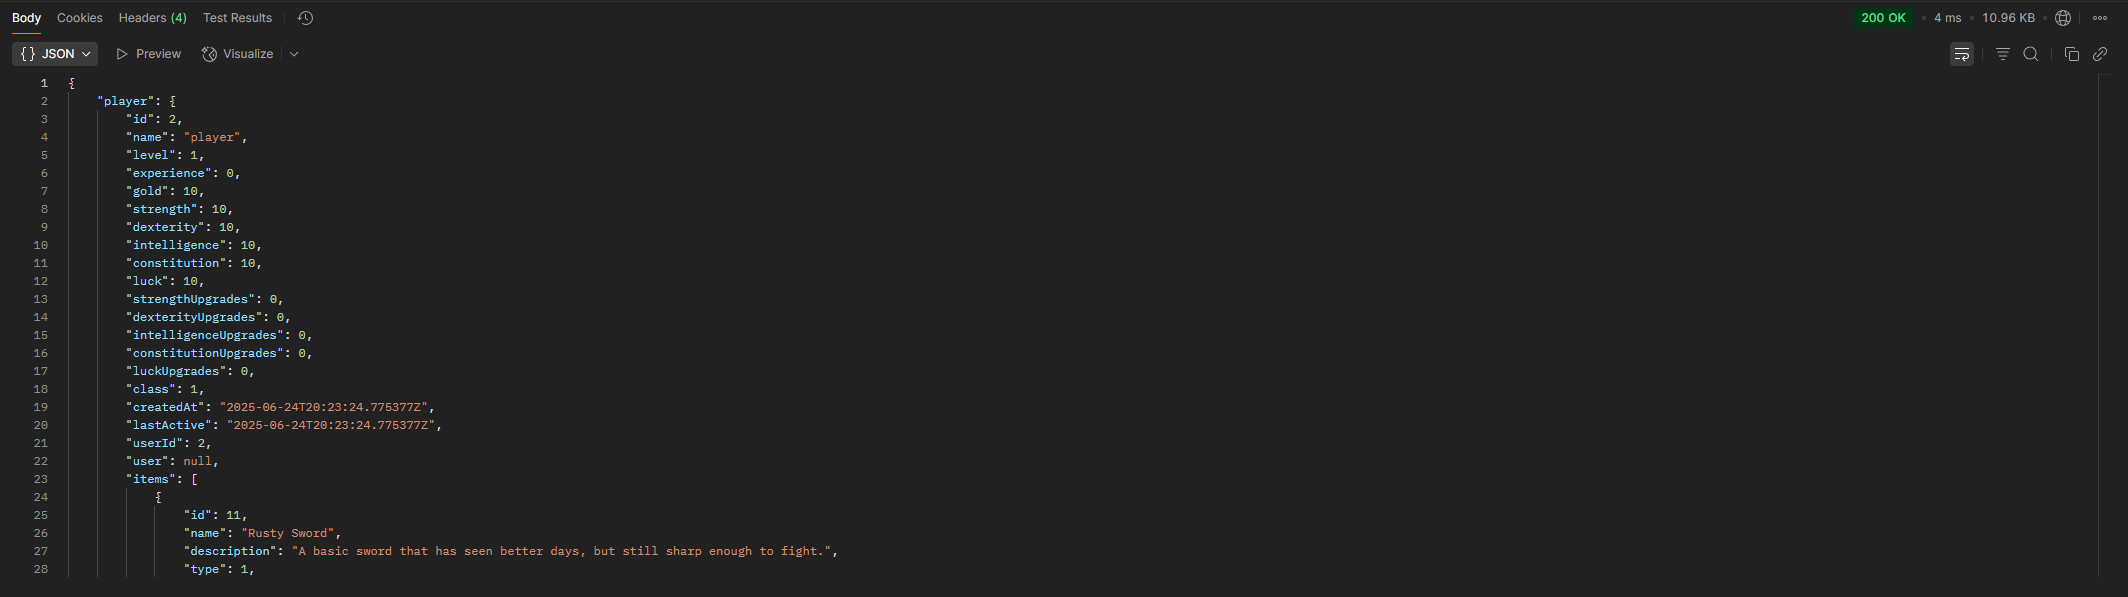
\includegraphics[width=480px]{figures/testy/test-completequest.png}
            \caption{Test zakończenia misji}
        \end{figure}
    \end{itemize}

    \item \textbf{Obsługa nieautoryzowanego dostępu}
    \begin{itemize}
        \item \textbf{Cel:} Sprawdzenie, czy API odrzuca żądania bez ważnego tokenu.
        \item \textbf{Warunki początkowe:} Brak tokenu lub token nieprawidłowy.
        \item \textbf{Kroki testowe:}
        \begin{enumerate}
            \item Wysłanie żądania GET /api/players/me bez nagłówka Authorization.
        \end{enumerate}
        \item \textbf{Dane wejściowe:} Brak lub nieprawidłowy token.
        \item \textbf{Oczekiwany rezultat:} Odpowiedź 401 Unauthorized.
        \item \textbf{Wynik testu:}
        \begin{figure}[H]
            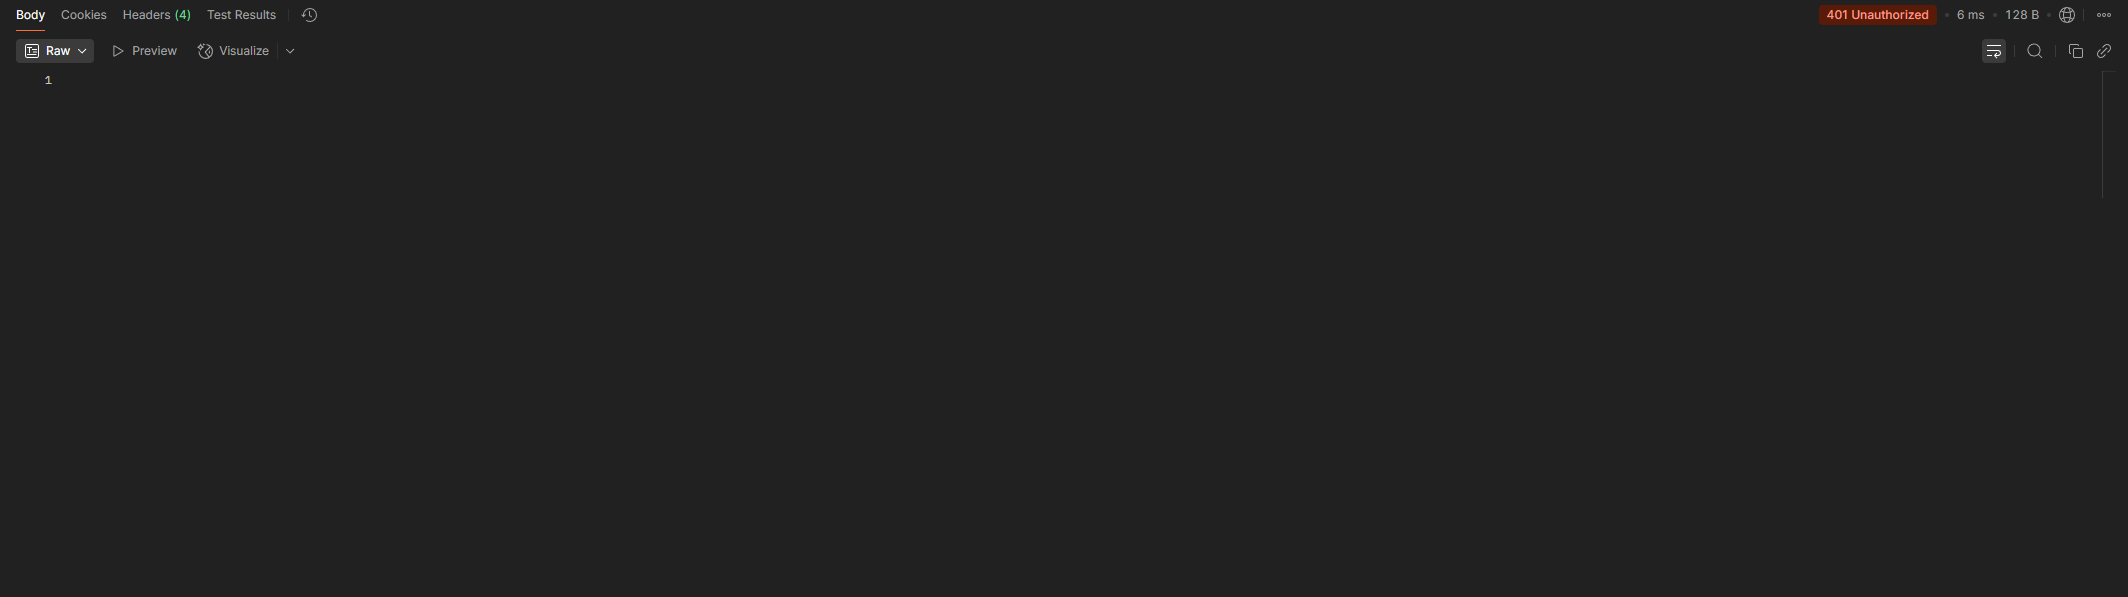
\includegraphics[width=480px]{figures/testy/test-unauthorized.png}
            \caption{Test nieautoryzowanego dostępu}
        \end{figure}
    \end{itemize}
\end{itemize}

\section{Testy frontendu (UI)}

\begin{itemize}
    \item \textbf{Rejestracja użytkownika przez interfejs}
    \begin{itemize}
        \item \textbf{Cel:} Sprawdzenie poprawności działania formularza rejestracji.
        \item \textbf{Warunki początkowe:} Brak zalogowanego użytkownika.
        \item \textbf{Kroki testowe:}
        \begin{enumerate}
            \item Otwórz stronę rejestracji.
            \item Wprowadź dane użytkownika i zatwierdź formularz.
        \end{enumerate}
        \item \textbf{Dane wejściowe:} E-mail, hasło, nazwa użytkownika.
        \item \textbf{Oczekiwany rezultat:} Komunikat o sukcesie, przekierowanie do ekranu logowania lub gry.
        \item \textbf{Wynik testu:}
        \begin{figure}[H]
            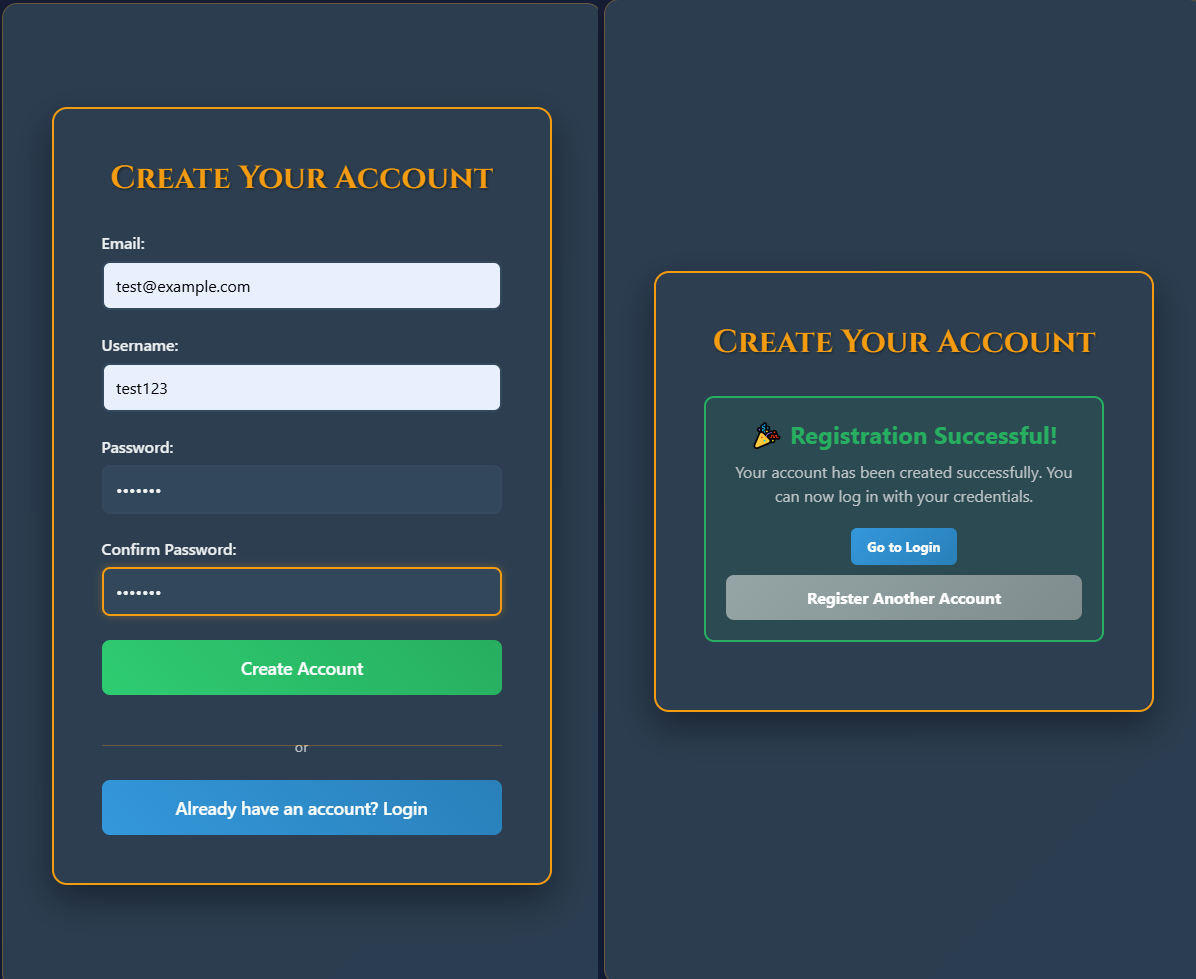
\includegraphics[width=480px]{figures/testy/test-registration-front.png}
            \caption{Test rejestracji użytkownika - frontend}
        \end{figure}
    \end{itemize}


    \item \textbf{Logowanie użytkownika przez interfejs}
    \begin{itemize}
        \item \textbf{Cel:} Sprawdzenie poprawności działania formularza logowania.
        \item \textbf{Warunki początkowe:} Istnieje zarejestrowany użytkownik.
        \item \textbf{Kroki testowe:}
        \begin{enumerate}
            \item Otwórz stronę logowania.
            \item Wprowadź poprawne dane i zatwierdź formularz.
        \end{enumerate}
        \item \textbf{Dane wejściowe:} E-mail, hasło.
        \item \textbf{Oczekiwany rezultat:} Przekierowanie do ekranu gry, widoczne dane gracza.
        \item \textbf{Wynik testu:}
        \begin{figure}[H]
            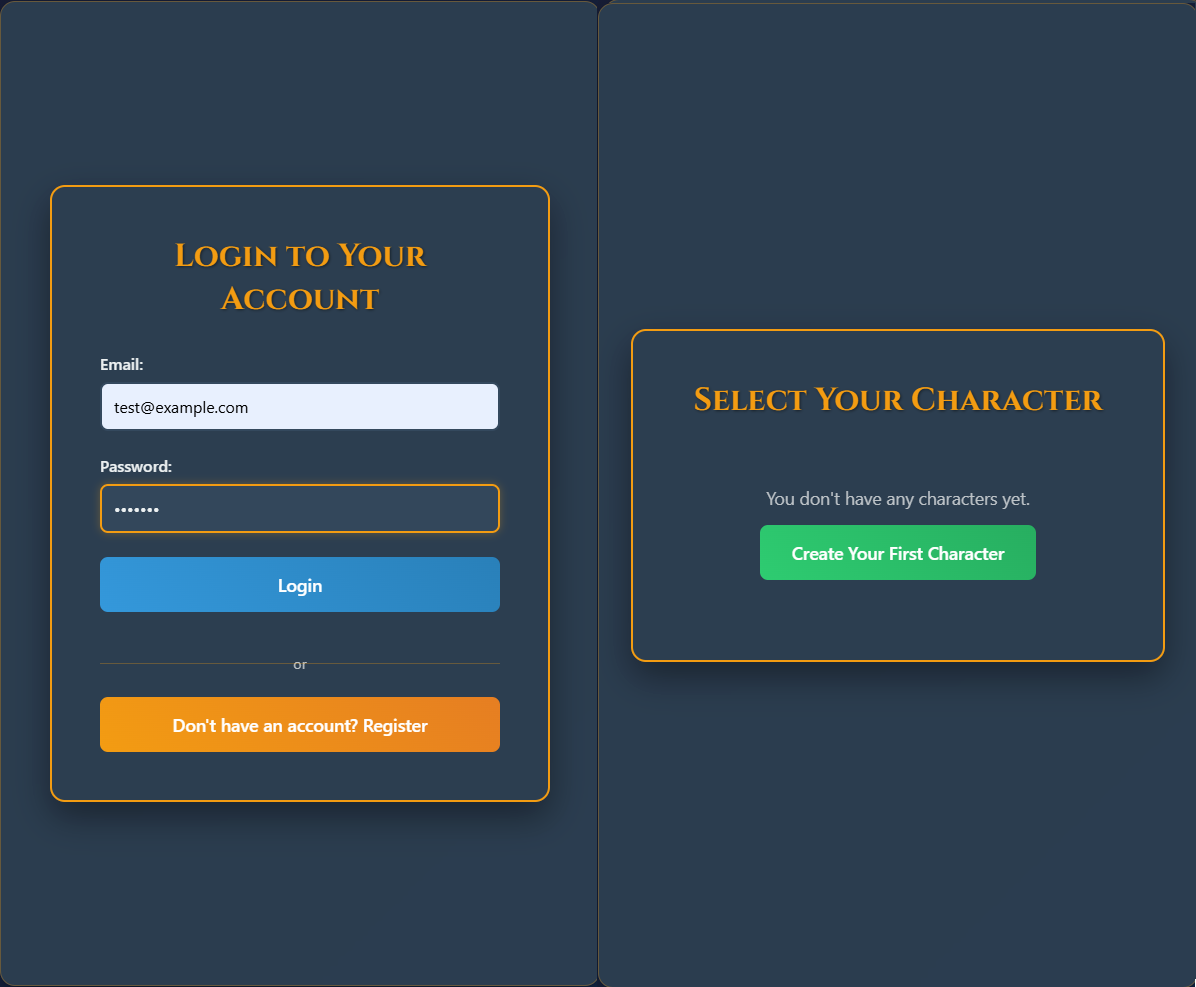
\includegraphics[width=480px]{figures/testy/test-login-front.png}
            \caption{Test logowania użytkownika - frontend}
        \end{figure}
    \end{itemize}

    \item \textbf{Wyświetlanie ekwipunku gracza}
    \begin{itemize}
        \item \textbf{Cel:} Sprawdzenie poprawności wyświetlania ekwipunku po zalogowaniu.
        \item \textbf{Warunki początkowe:} Gracz jest zalogowany, posiada przedmioty.
        \item \textbf{Kroki testowe:}
        \begin{enumerate}
            \item Przejdź do ekranu ekwipunku.
        \end{enumerate}
        \item \textbf{Dane wejściowe:} Token JWT (w tle).
        \item \textbf{Oczekiwany rezultat:} Lista przedmiotów widoczna na ekranie.
        \item \textbf{Wynik testu:}
        \begin{figure}[H]
            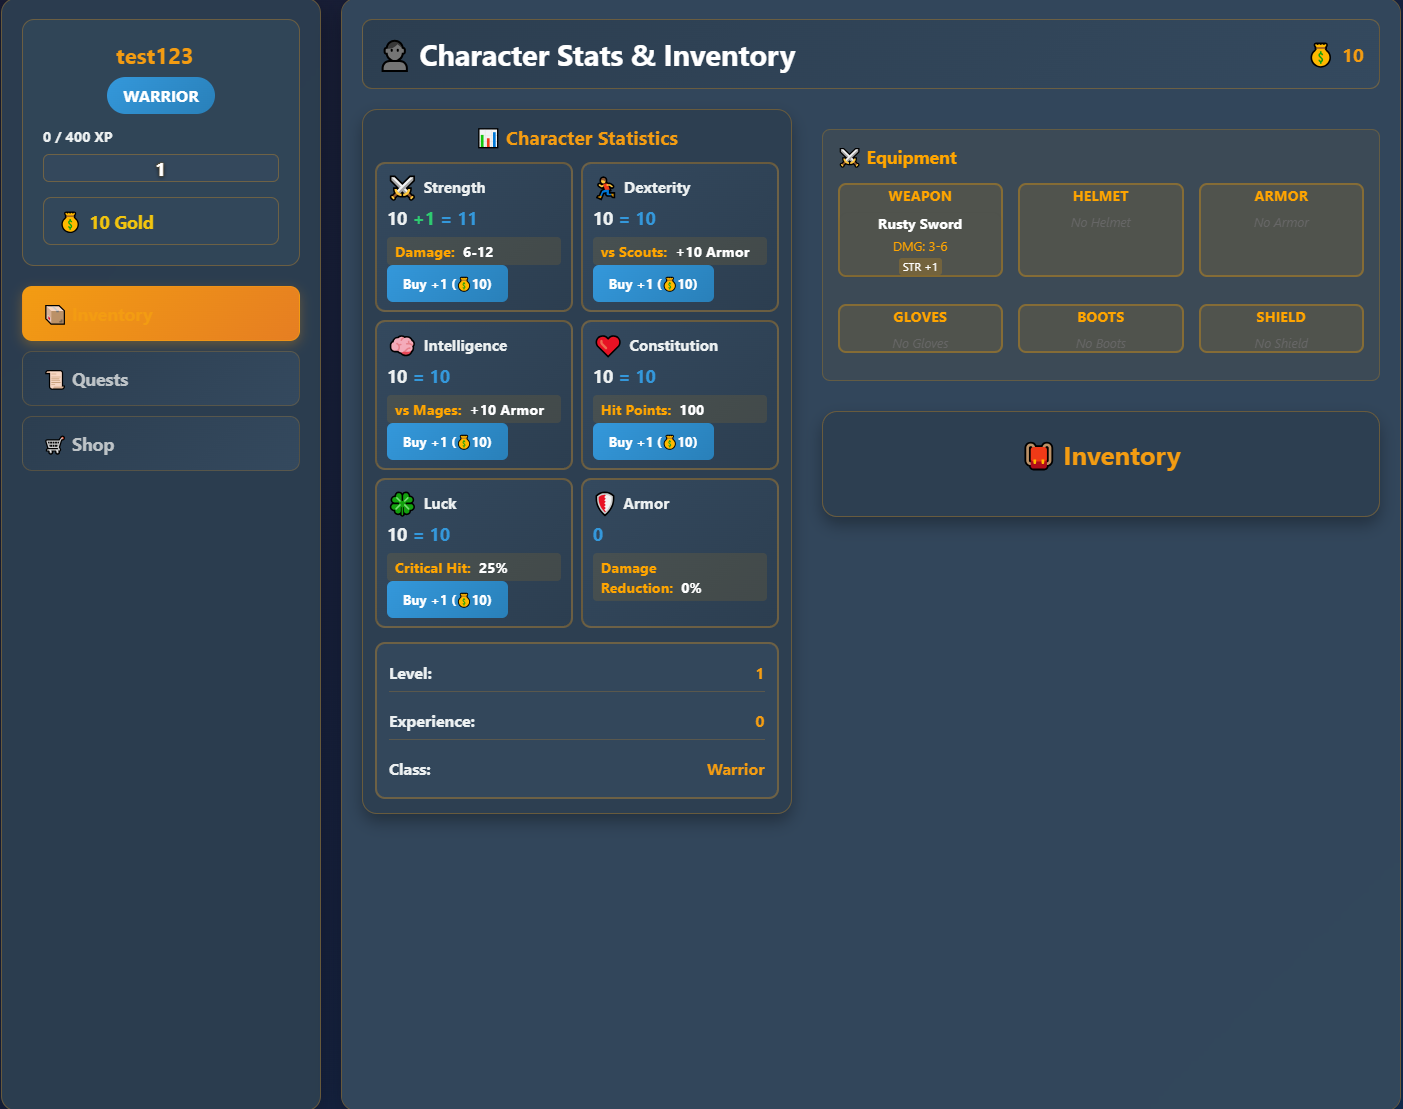
\includegraphics[width=480px]{figures/testy/test-inventory-front.png}
            \caption{Test ekwipunku gracza}
        \end{figure}
    \end{itemize}

    \item \textbf{Zakup przedmiotu przez interfejs}
    \begin{itemize}
        \item \textbf{Cel:} Sprawdzenie możliwości zakupu przedmiotu przez UI.
        \item \textbf{Warunki początkowe:} Gracz jest zalogowany, ma wystarczającą ilość złota.
        \item \textbf{Kroki testowe:}
        \begin{enumerate}
            \item Przejdź do sklepu.
            \item Wybierz przedmiot i kliknij "Kup".
        \end{enumerate}
        \item \textbf{Dane wejściowe:} Identyfikator przedmiotu (wybór w UI).
        \item \textbf{Oczekiwany rezultat:} Przedmiot pojawia się w ekwipunku, złoto zmniejszone.
        \item \textbf{Wynik testu:}
        \begin{figure}[H]
            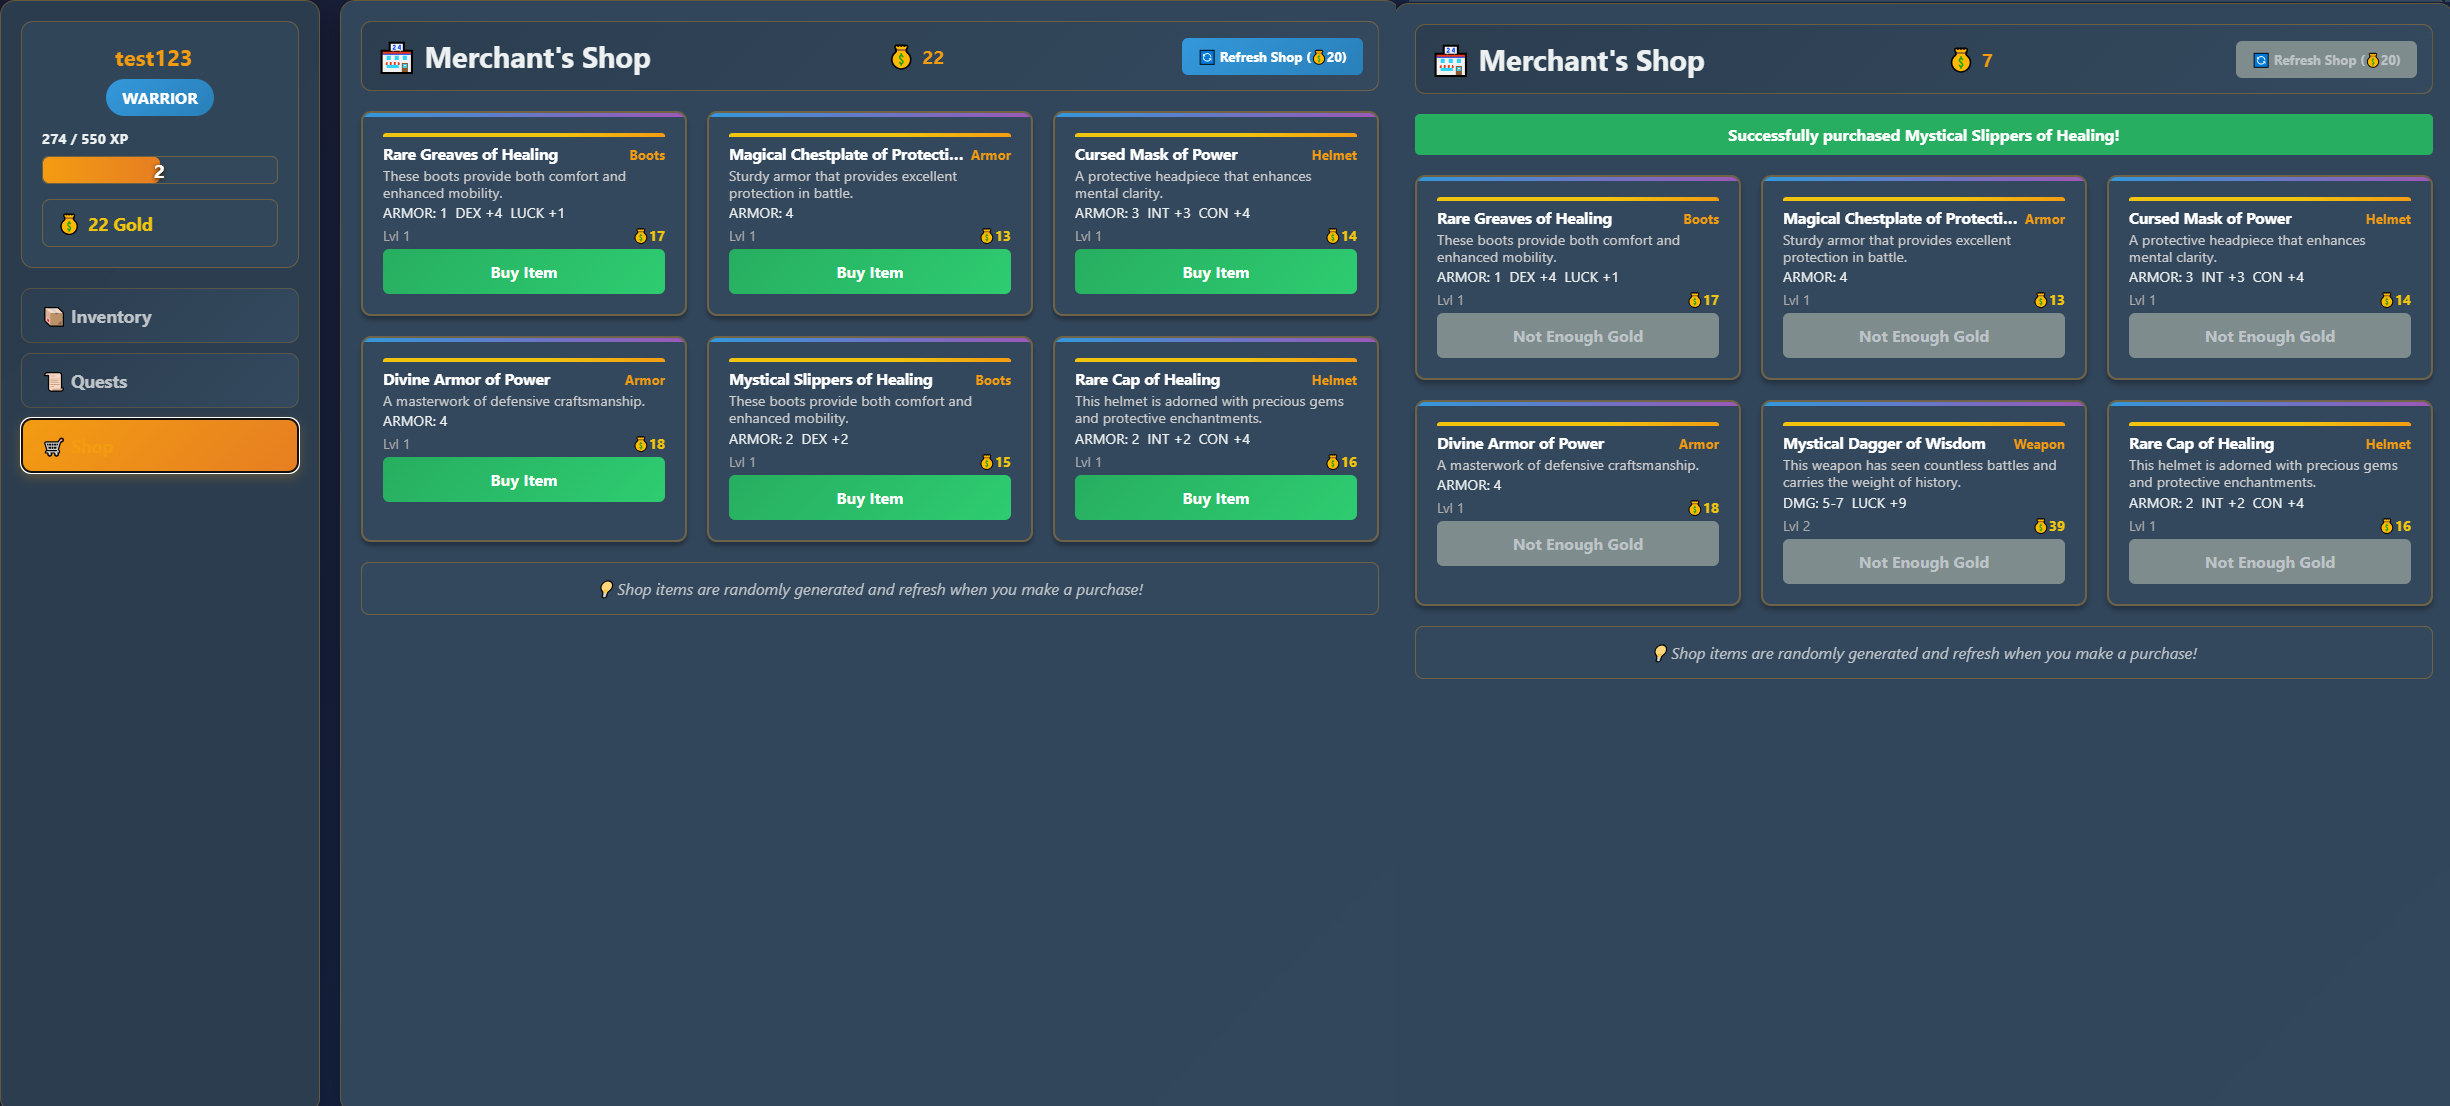
\includegraphics[width=480px]{figures/testy/test-buyitem-front.png}
            \caption{Test zakupu przedmiotu - frontend}
        \end{figure}
    \end{itemize}

    \item \textbf{Rozpoczęcie i zakończenie misji przez interfejs}
    \begin{itemize}
        \item \textbf{Cel:} Sprawdzenie poprawności obsługi misji przez UI.
        \item \textbf{Warunki początkowe:} Gracz jest zalogowany, ma dostępne misje.
        \item \textbf{Kroki testowe:}
        \begin{enumerate}
            \item Przejdź do tablicy misji.
            \item Wybierz misję i kliknij "Rozpocznij".
            \item Po zakończeniu kliknij "Odbierz nagrodę".
        \end{enumerate}
        \item \textbf{Dane wejściowe:} Identyfikator misji (wybór w UI).
        \item \textbf{Oczekiwany rezultat:} Misja znika z listy aktywnych, nagroda pojawia się w ekwipunku.
        \item \textbf{Wynik testu:}
        \begin{figure}[H]
            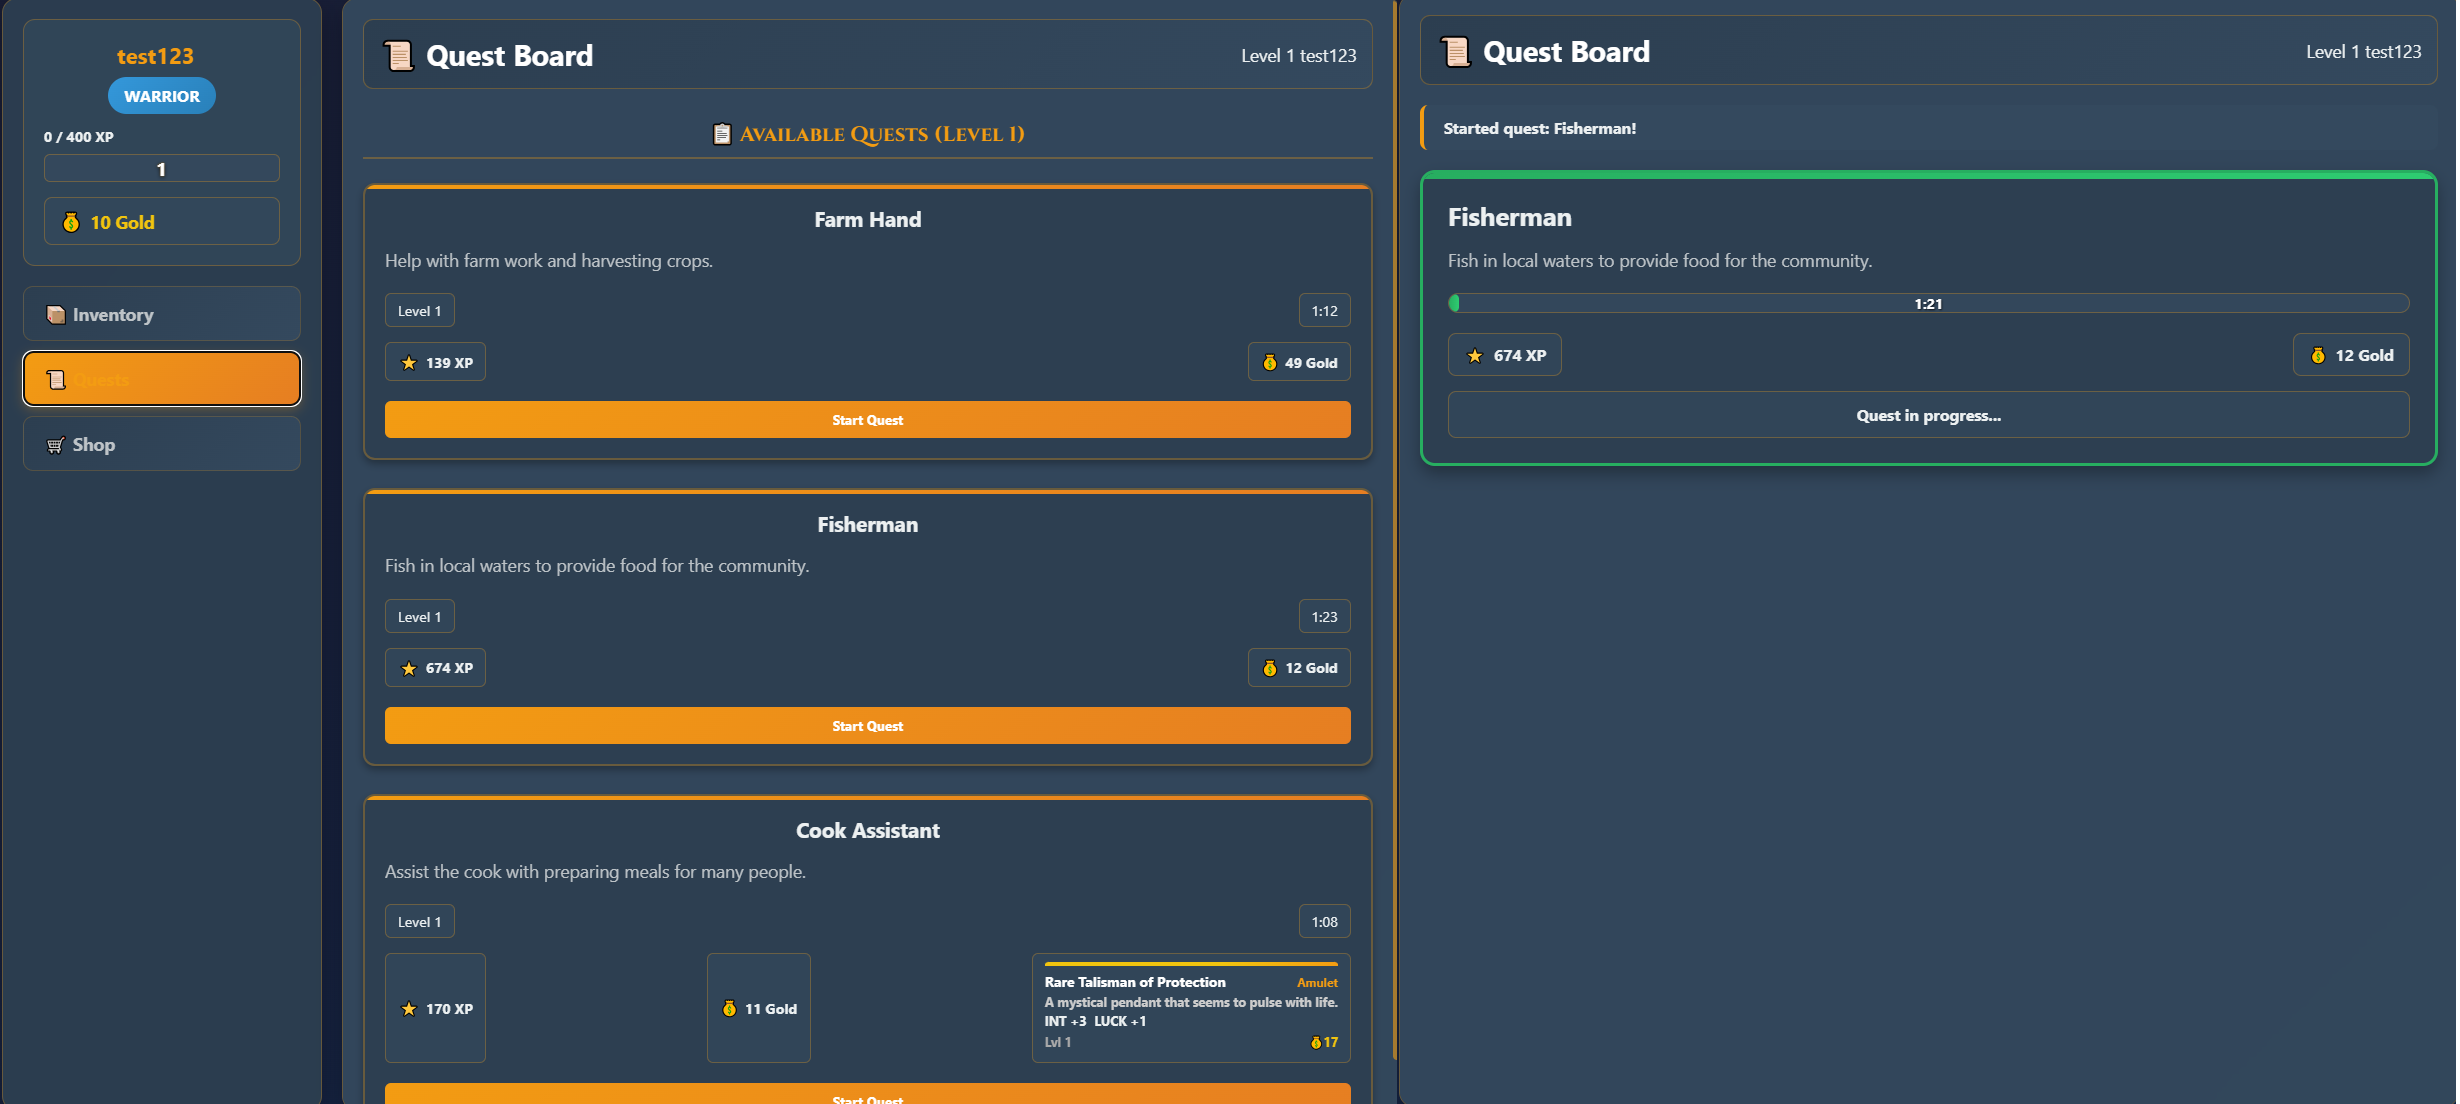
\includegraphics[width=480px]{figures/testy/test-startquest-front.png}
            \caption{Test rozpoczęcia misji}
        \end{figure}
        \begin{figure}[H]
            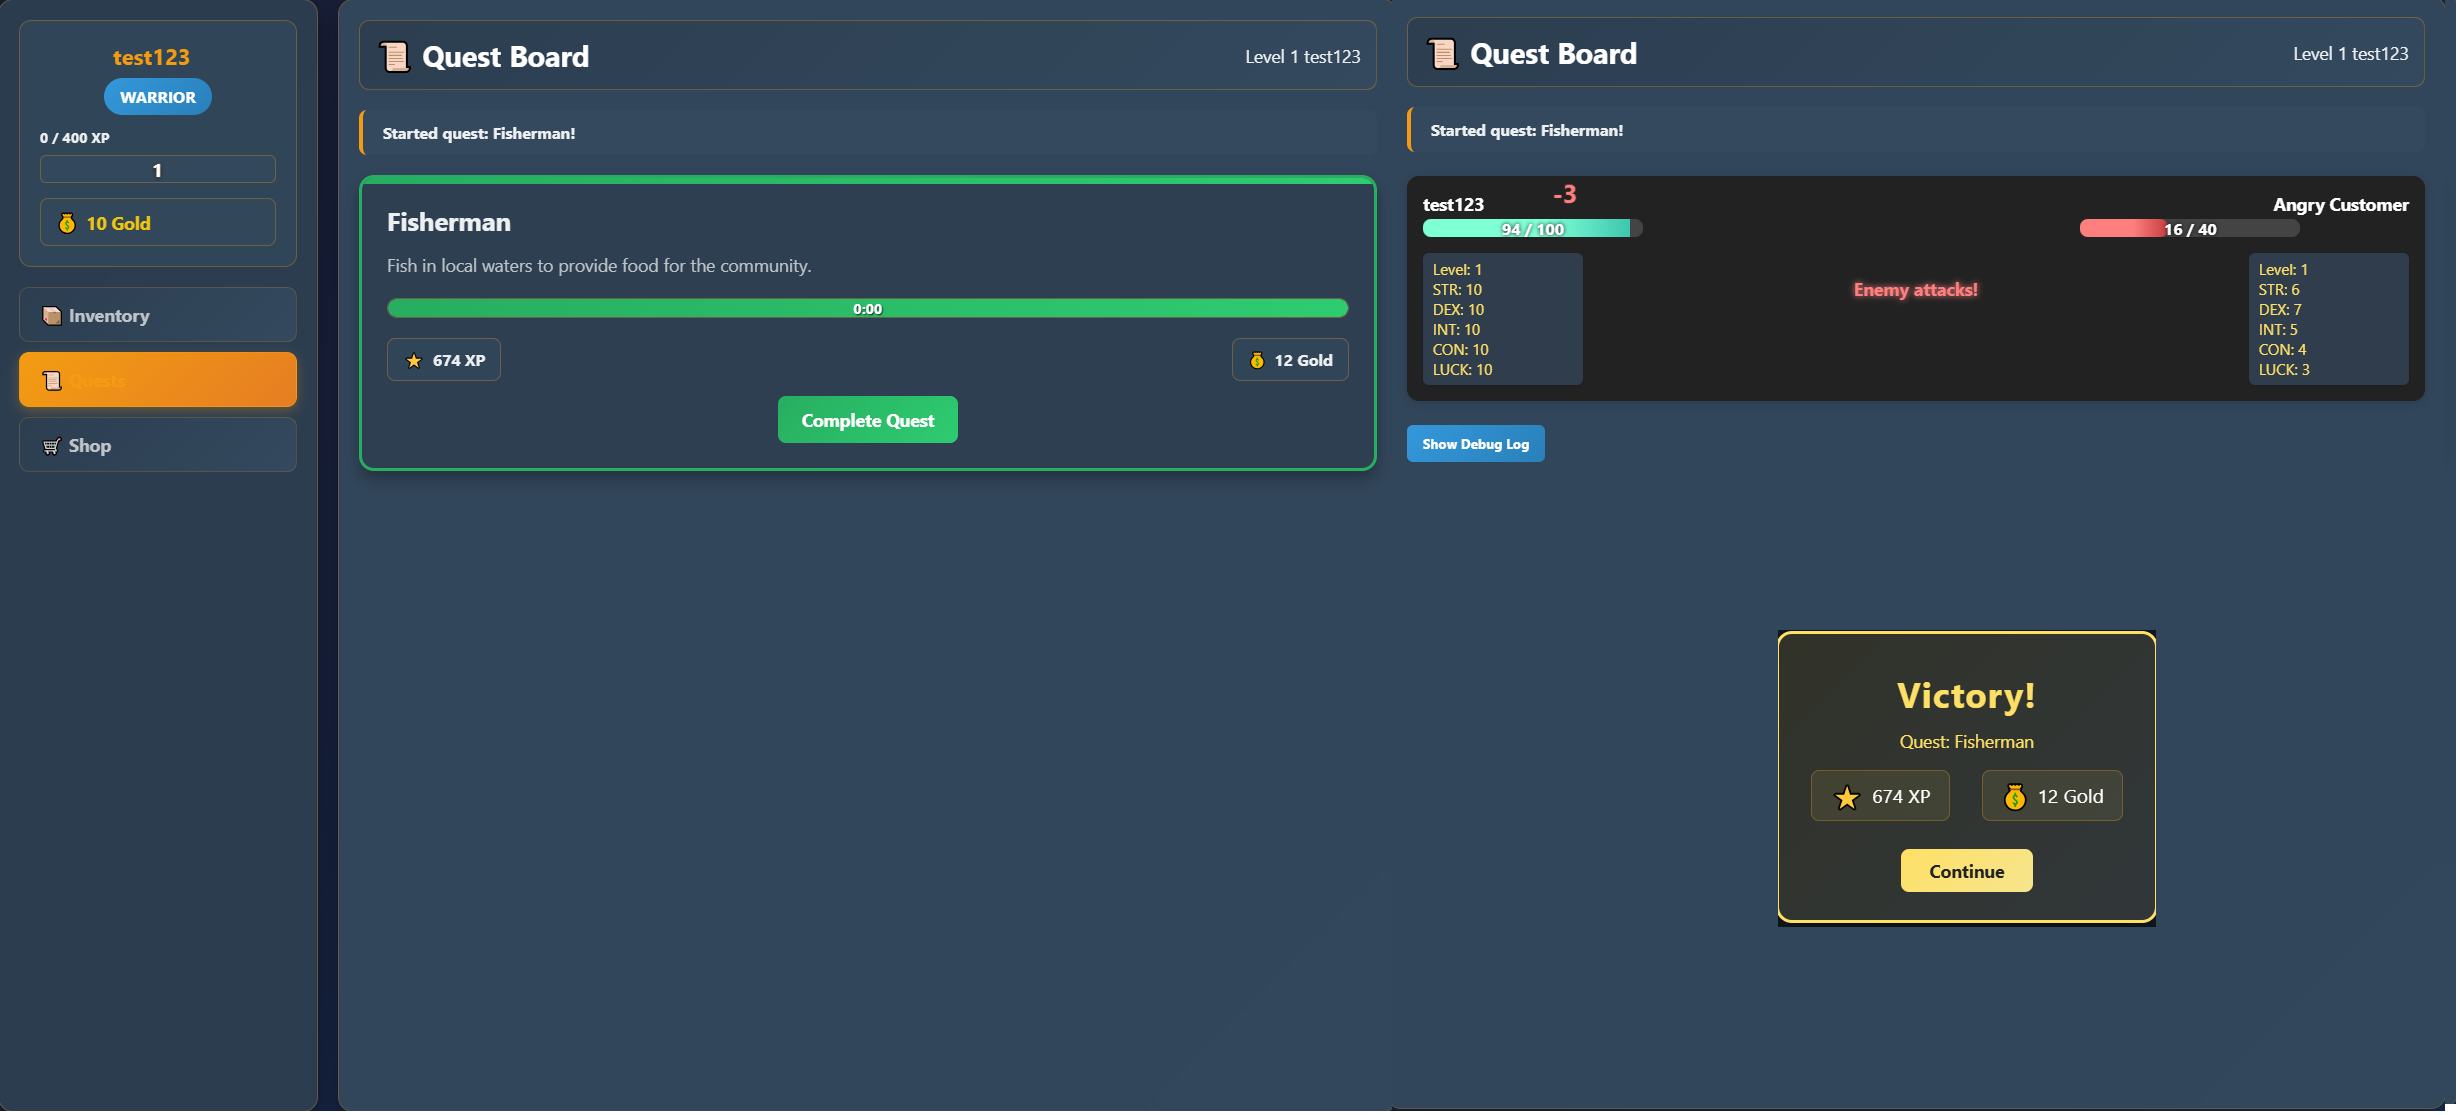
\includegraphics[width=480px]{figures/testy/test-completequest-front.png}
            \caption{Test zakończenia misji}
        \end{figure}
    \end{itemize}

    \item \textbf{Ulepszenie statystyk przez interfejs}
    \begin{itemize}
        \item \textbf{Cel:} Sprawdzenie możliwości ulepszania statystyk przez UI.
        \item \textbf{Warunki początkowe:} Gracz jest zalogowany, ma wystarczającą ilość złota.
        \item \textbf{Kroki testowe:}
        \begin{enumerate}
            \item Przejdź do ekranu statystyk.
            \item Kliknij przycisk ulepszenia wybranej statystyki.
        \end{enumerate}
        \item \textbf{Dane wejściowe:} Nazwa statystyki (wybór w UI).
        \item \textbf{Oczekiwany rezultat:} Statystyka zwiększona, złoto zmniejszone.
        \item \textbf{Wynik testu:}
        \begin{figure}[H]
            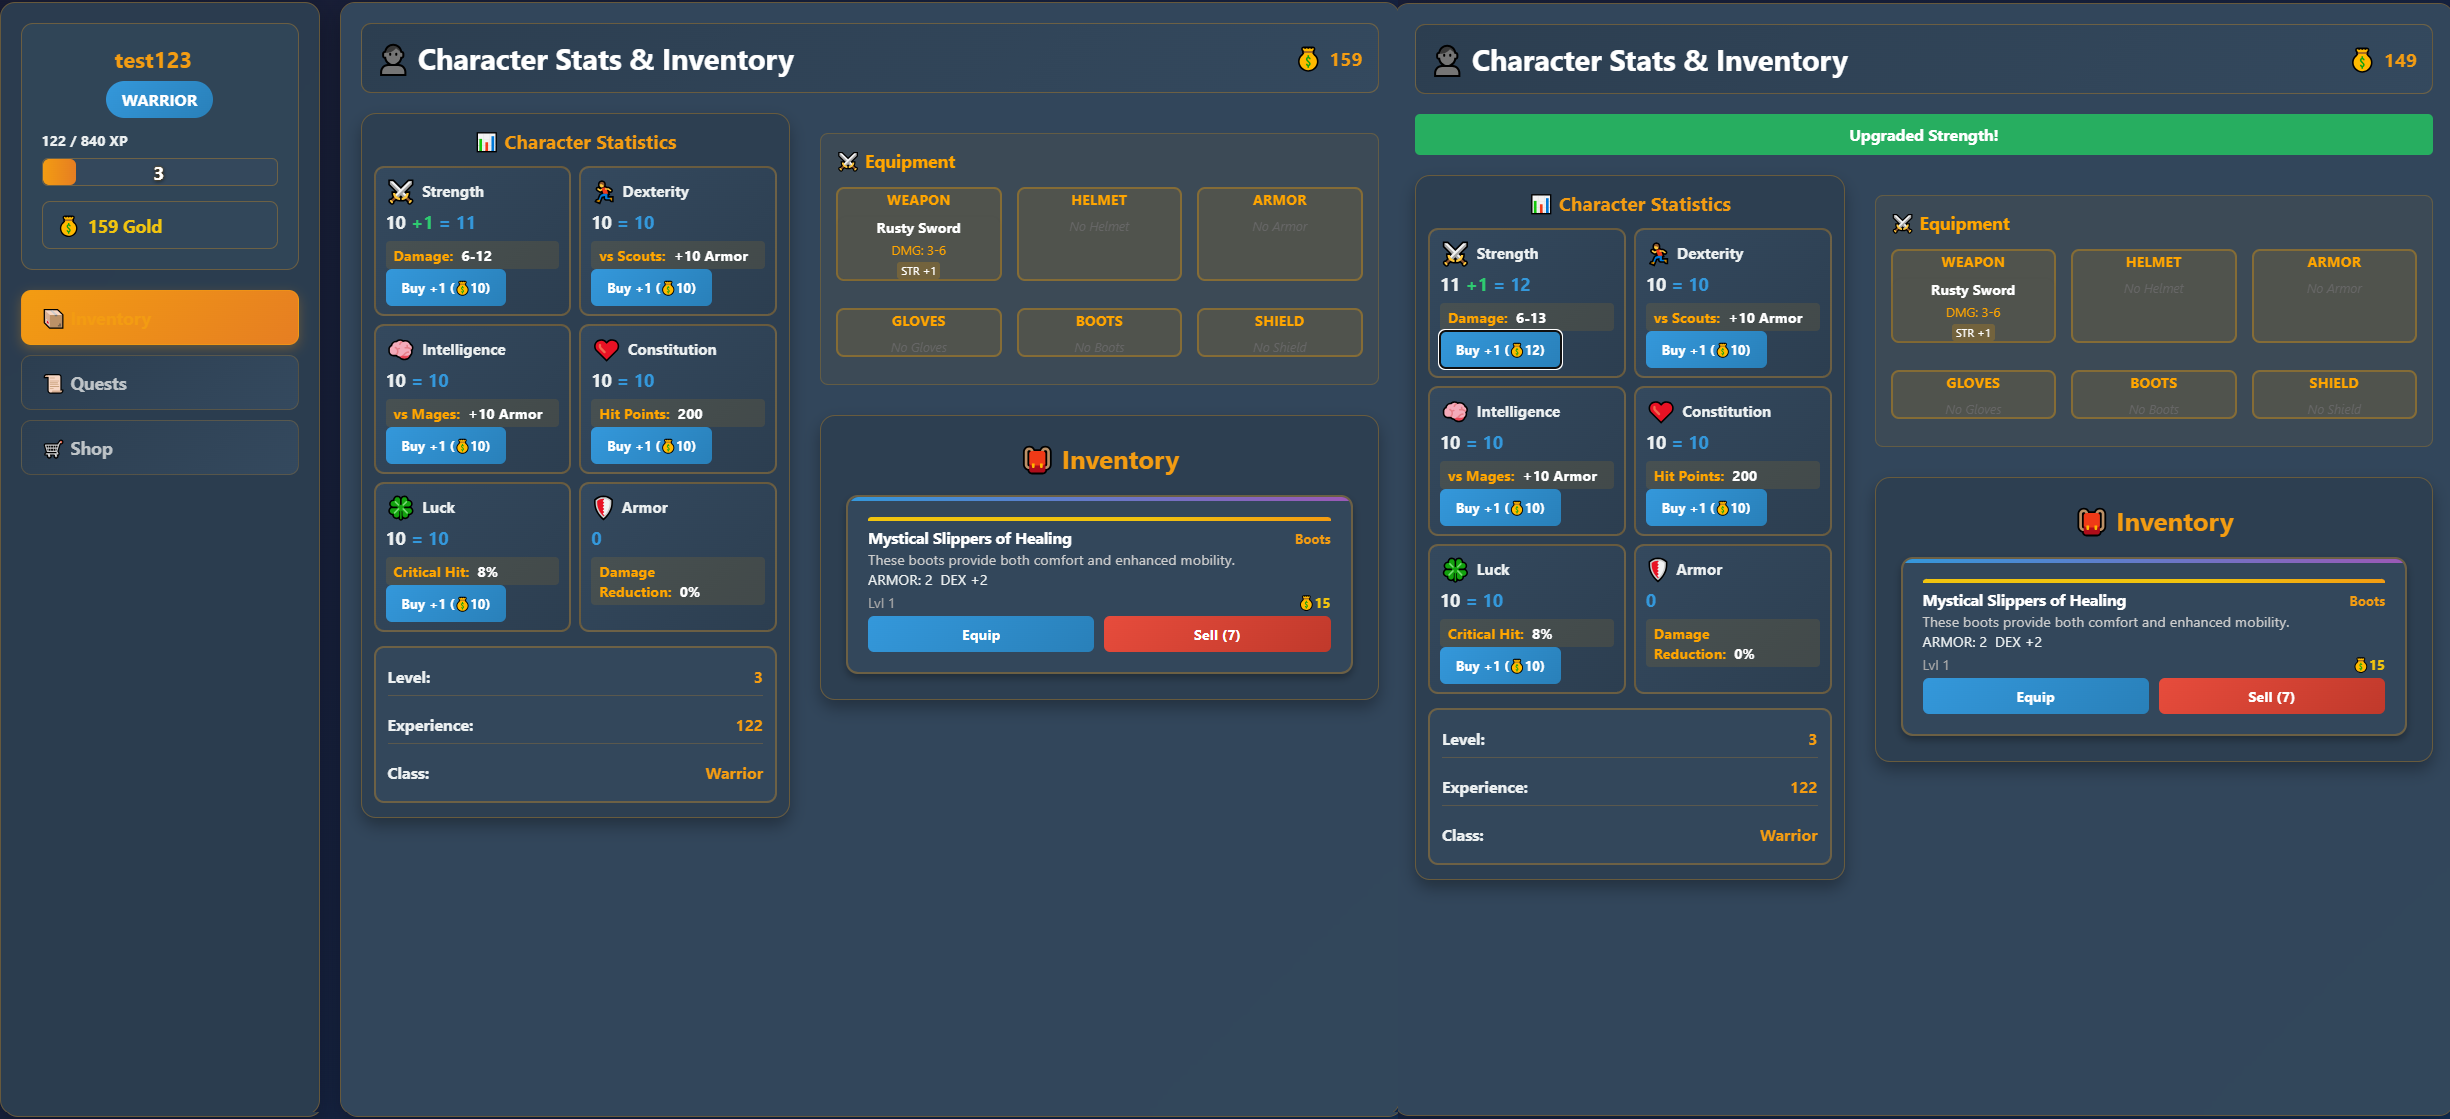
\includegraphics[width=480px]{figures/testy/test-upgradestat-front.png}
            \caption{Test ulepszenia statystyk}
        \end{figure}
    \end{itemize}
\end{itemize}



% ********** Koniec rozdziału **********